\documentclass[twoside,a4paper,12pt]{book}%,AutoFakeBold,twoside,openright,
% 可用选项有 debug|ebook|hardcopy, amd|pmd|phdplain|phdfancy, nobox, manualSpine, onlyCover, twoSideCover, noBlankPages.
% debug 生成的PDF带框线,方便调试
% ebook 带彩色文字的PDF
% hardcopy 无彩色文字的PDF
% amd 学硕使用
% pmd 专硕使用
% phdplain 博士论文简装
% phdfancy 博士论文精装
% nobox 输出的封面无框线和书脊
% manualSpine 手动输出书脊,需配合\jluManualSpine命令
% onlyCover 仅输出封面页
% twoSideCover 输出双页封面
% noBlankPages 去掉空白页,主要用于上传到图书馆学位论文系统
% 默认为 hardcopy,amd,且nobox=false,manualSpine=false,onlyCover=false,twoSideCover=false, noBlankPages=false
% 双面印刷需在documentclass选项中声明twoside
% 单面印刷需在documentclass选项中声明oneside
% 选项使用举例如下
%\usepackage[phdplain,ebook,twoSideCover,onlyCover]{jluthesis2020}%
%\usepackage[amd,hardcopy,twoSideCover]{jluthesis2020}%
\usepackage[phdplain,hardcopy,noBlankPages]{jluthesis2020}%

% 用于算法注释
\usepackage{algcompatible}
\renewcommand{\COMMENT}[2][.5\linewidth]{%
  \leavevmode\hfill\makebox[#1][l]{//~#2}}
\algnewcommand\algorithmicto{\textbf{to}}
\algnewcommand\RETURN{\State \textbf{return} }

% 用于排版代码
\usepackage{listings}


\graphicspath{{figures/}}

\newcommand{\Title}{吉林大学学位论文模板{\jluthesisVersion}示例}
\newcommand{\Author}{千颂伊}

\begin{document}
\frontmatter
\sloppy % 解决中英文混排的断行问题,会加入间距,但不会影响断行 ????


% 手动在长标题中利用 \par 输入断行,
\jluCTitle{\Title}

% 竖排的书脊输出时,如果遇到中英混杂的标题会比较麻烦,需要中英分开控制输出
% 但如果仅有中文或英文都比较简单,如
% \jluCSpineTitle{吉林大学学位论文模版示例} % 仅中文的书脊标题
% \jluCSpineTitle{\jluPrintSpine{Sample Typesetting for {\jluthesisVersion}}} % 仅英文的书脊标题
\jluCSpineTitle{\jluPrintSpine{\jluPrintSpineChinese{吉林大学学位论文模版}{\jluthesisVersion}\jluPrintSpineChinese{示例}}} % 中英混杂的书脊标题

\jluSpineHorizontalPosition{1.65} % 书脊的水平位置,修改可使书脊水平平移

% 当在选项中指定手动输出书脊时,可用下列命令手动输出书脊进行微调
% \jluManualSpine{
%   % for oneSideCover
%	\jluPrintVerticallyOneByOne{2.5cm}{-10em}{吉林大学学位论文模板}{0.2in}{}
%	\jluPrintVerticallySentence{2.5cm}{-26.5em}{\rotatebox{-90}{\jluthesisVersion}}
%	\jluPrintVerticallyOneByOne{2.5cm}{-30em}{示例}{0.2in}{}
%	\jluPrintVerticallyOneByOne{2.45cm}{-38em}{ \Author }{0.2in}{\bfseries}
%	\jluPrintVerticallyOneByOne{2.5cm}{-47em}{ 吉林大学 }{0.2in}{\kai}
%   % for twoSideCover    
%	\jluPrintVerticallyOneByOne{23cm}{-10em}{吉林大学学位论文模板}{0.2in}{}
%	\jluPrintVerticallySentence{23cm}{-26.5em}{\rotatebox{-90}{\jluthesisVersion}}
%	\jluPrintVerticallyOneByOne{23cm}{-30em}{示例}{0.2in}{}
%	\jluPrintVerticallyOneByOne{23cm}{-38em}{ \Author }{0.2in}{\bfseries}
%	\jluPrintVerticallyOneByOne{23cm}{-47em}{ 吉林大学 }{0.2in}{\kai}
% } % jluManualSpine
\jluETitle{Sample Typesetting for {\jluthesisVersion}}
\jluCSubject{计算机应用技术}   % 封面的『专业』或『类别』
\jluCInterest{数据挖掘}  % 封面的『研究方向』或『领域(方向)』,博士精装版扉页的『研究方向』
\jluCSubjectScd{计算机应用技术}  % 扉页的『专业名称』或『领域(方向)』
\jluCSubjectTrd{计算机应用技术}  % 学位论文授权说明中的『学科专业』
\jluCDegree{工学硕士}  % 扉页的『学位类别』或『类别』
\jluCCollege{计算机科学与技术学院}
\jluCollegeNumber{10183}
\jluCUniversity{吉林大学}
\jluCAuthor{\Author} % 若为两个字建议中间留一个汉字的空间,如王\hphantom{空}喆
\jluCSupervisor{都敏俊} % 若为两个字建议中间留一个汉字的空间,如王\hphantom{空}喆
\jluCSupervisorPost{教授}
\jluClassification{TP391}
\jluSecurityLevel{公开}
\jluCAddress{吉林大学计算机科学与技术学院,130012} 
\jluTelphone{(+86) 1884454XXXX}  
\jluStudentNumber{201753XXXX}

\jluAuthorSignatureOne{ % 原创声明作者签名
	\raisebox{0.5cm}{
		\hspace{3.5cm}
		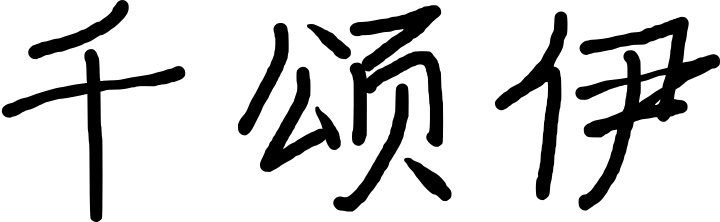
\includegraphics[width=3cm]{qian-song-yi.png}	
	}
}
\jluAuthorSignatureTwo{ % 授权声明作者签名
	\raisebox{0.5cm}{
		\hspace{3.5cm}
		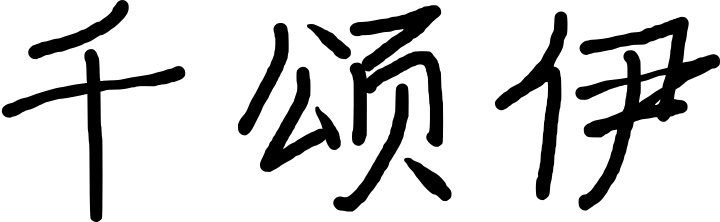
\includegraphics[width=3cm]{qian-song-yi.png}	
	}
}
\jluSupervisorSignature{ % 授权声明导师签名
	\raisebox{0.5cm}{
		\hspace{3.5cm}
		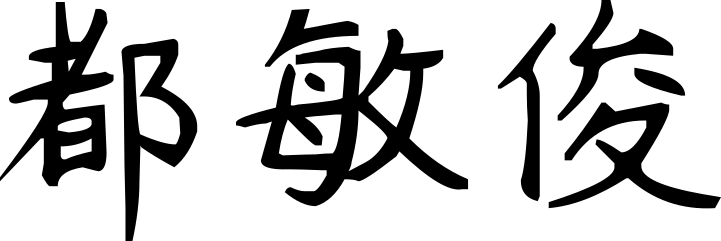
\includegraphics[width=3cm]{du-min-jun.png}
	}
}

% 以下日期若注释掉,对应的日期将留空
\jluDateForCover{2020}{4}
\jluDegreeObtainDate{2020}{6}{21}
\jluDefenseDate{2020}{5}{31}
\jluOriginalStatementDate{2020}{6}{1}
\jluContributionStatementDate{2020}{6}{1}

\jluCommitteeTable{
	%\vspace{5cm}
	\setstretch{1.32}
    \begin{tabular}{l@{\hspace{0.5cm}}l@{\hspace{1.0cm}}l@{\hspace{1.5cm}}r}
    \multicolumn{4}{l}{答辩委员会组成:}\\
            &姓名 & 职称 & 工作单位 \\
        主席&徐宜花& 教授 & XX大学   \\
        委员&李辉京& 教授 & YYYY大学   \\
           &刘世美& 教授 & ZZZZZZZZ大学   \\
           &千允才& 教授 & AA大学   \\
           &张英牧& 教授 & BB大学   \\
           &尹\quad 凡& 研究员 & BB大学   \\
    \end{tabular}
}

\jluCAbstract{
   电子计算机(亦稱电脑)是利用数字电子技术,根据一系列指令指示並且自动执行任意算术或逻辑操作序列的设备。通用计算机因有能遵循被称为“程序”的一般操作集的能力而使得它们能够执行极其广泛的任务。

计算机被用作各种工业和消费设备的控制系统。这包括简单的特定用途设备(如微波炉和遥控器)、工业设备(如工业机器人和计算机辅助设计),及通用设备(如个人电脑和智能手机之类的移动设备)等。尽管计算机种类繁多,但根据图灵机理论,一部具有著基本功能的计算机,应当能够完成任何其它计算机能做的事情。因此,理论上从智能手机到超级计算机都应该可以完成同样的作业(不考虑时间和存储因素)。由于科技的飞速进步,下一代计算机总是在性能上能够显著地超过其前一代,这一现象有时被称作“摩尔定律”。通过互联网,计算机互相连接,极大地提高了信息交换速度,反过来推动了科技的发展。在21世纪的现在,计算机的应用已经涉及到方方面面,各行各业了。

自古以来,简单的手动设备——就像算盘——帮助人们进行计算。在工业革命初期,各式各样机械的出现,而初衷都是为了自动完成冗长而乏味的任务,例如织机的编织图案。更复杂的机器在20世纪初出现,通过模拟电路进行复杂特定的计算。第一台数字电子计算机出现于二战期间。自那时以来,电脑的速度,功耗和多功能性則不断增加。在现代,机械计算机的应用已经完全被电子计算机所取代。

计算机在组成上形式不一,早期计算机的天依然有大量体积庞大的巨型计算机为特别的科学计算或面向大型组织的事务处理需求服务。比较小的,为个人应用而设计的称为微型计算机(Personal Computer,PC),在中國地區简称為「微机」。我們今天在日常使用“计算机”一词时通常也是指此,不过现在计算机最为普遍的应用形式却是嵌入式,嵌入式计算机通常相对简单、体积小,并被用来控制其它设备——无论是飞机、工业机器人还是数码相机。

同计算机相关的技术研究叫電腦科學,而「计算机技术」指的是将计算机科学的成果应用于工程实践所派生的诸多技术性和经验性成果的总合。「计算机技术」与「计算机科学」是两个相关而又不同的概念,它们的不同在于前者偏重于实践而后者偏重于理论。至於由数据为核心的研究則称為信息技术。

传统上,现代计算机包含至少一个处理单元(通常是中央处理器(CPU))和某种形式的存储器。处理元件执行算术和逻辑运算,并且排序和控制单元可以响应于存储的信息改变操作的顺序。外围设备包括输入设备(键盘,鼠标,操纵杆等)、输出设备(显示器屏幕,打印机等)以及执行两种功能(例如触摸屏)的输入/输出设备。外围设备允许从外部来源检索信息,并使操作结果得以保存和检索。

电子计算机(亦稱电脑)是利用数字电子技术,根据一系列指令指示並且自动执行任意算术或逻辑操作序列的设备。通用计算机因有能遵循被称为“程序”的一般操作集的能力而使得它们能够执行极其广泛的任务。

计算机被用作各种工业和消费设备的控制系统。这包括简单的特定用途设备(如微波炉和遥控器)、工业设备(如工业机器人和计算机辅助设计),及通用设备(如个人电脑和智能手机之类的移动设备)等。尽管计算机种类繁多,但根据图灵机理论,一部具有著基本功能的计算机,应当能够完成任何其它计算机能做的事情。因此,理论上从智能手机到超级计算机都应该可以完成同样的作业(不考虑时间和存储因素)。由于科技的飞速进步,下一代计算机总是在性能上能够显著地超过其前一代,这一现象有时被称作“摩尔定律”。通过互联网,计算机互相连接,极大地提高了信息交换速度,反过来推动了科技的发展。在21世纪的现在,计算机的应用已经涉及到方方面面,各行各业了。

自古以来,简单的手动设备——就像算盘——帮助人们进行计算。在工业革命初期,各式各样机械的出现,而初衷都是为了自动完成冗长而乏味的任务,例如织机的编织图案。更复杂的机器在20世纪初出现,通过模拟电路进行复杂特定的计算。第一台数字电子计算机出现于二战期间。自那时以来,电脑的速度,功耗和多功能性則不断增加。在现代,机械计算机的应用已经完全被电子计算机所取代。

计算机在组成上形式不一,早期计算机的天依然有大量体积庞大的巨型计算机为特别的科学计算或面向大型组织的事务处理需求服务。比较小的,为个人应用而设计的称为微型计算机(Personal Computer,PC),在中國地區简称為「微机」。我們今天在日常使用“计算机”一词时通常也是指此,不过现在计算机最为普遍的应用形式却是嵌入式,嵌入式计算机通常相对简单、体积小,并被用来控制其它设备——无论是飞机、工业机器人还是数码相机。

同计算机相关的技术研究叫電腦科學,而「计算机技术」指的是将计算机科学的成果应用于工程实践所派生的诸多技术性和经验性成果的总合。「计算机技术」与「计算机科学」是两个相关而又不同的概念,它们的不同在于前者偏重于实践而后者偏重于理论。至於由数据为核心的研究則称為信息技术。

传统上,现代计算机包含至少一个处理单元(通常是中央处理器(CPU))和某种形式的存储器。处理元件执行算术和逻辑运算,并且排序和控制单元可以响应于存储的信息改变操作的顺序。外围设备包括输入设备(键盘,鼠标,操纵杆等)、输出设备(显示器屏幕,打印机等)以及执行两种功能(例如触摸屏)的输入/输出设备。外围设备允许从外部来源检索信息,并使操作结果得以保存和检索。
}

\jluCKeywords{甲, 乙, 丙}

\jluEAbstract{
   A computer is a machine that can be instructed to carry out sequences of arithmetic or logical operations automatically via computer programming. Modern computers have the ability to follow generalized sets of operations, called programs. These programs enable computers to perform an extremely wide range of tasks. A ``complete'' computer including the hardware, the operating system (main software), and peripheral equipment required and used for ``full'' operation can be referred to as a computer system. This term may as well be used for a group of computers that are connected and work together, in particular a computer network or computer cluster.

Computers are used as control systems for a wide variety of industrial and consumer devices. This includes simple special purpose devices like microwave ovens and remote controls, factory devices such as industrial robots and computer-aided design, and also general purpose devices like personal computers and mobile devices such as smartphones. The Internet is run on computers and it connects hundreds of millions of other computers and their users.

Early computers were only conceived as calculating devices. Since ancient times, simple manual devices like the abacus aided people in doing calculations. Early in the Industrial Revolution, some mechanical devices were built to automate long tedious tasks, such as guiding patterns for looms. More sophisticated electrical machines did specialized analog calculations in the early 20th century. The first digital electronic calculating machines were developed during World War II. The first semiconductor transistors in the late 1940s were followed by the silicon-based MOSFET (MOS transistor) and monolithic integrated circuit (IC) chip technologies in the late 1950s, leading to the microprocessor and the microcomputer revolution in the 1970s. The speed, power and versatility of computers have been increasing dramatically ever since then, with MOS transistor counts increasing at a rapid pace (as predicted by Moore's law), leading to the Digital Revolution during the late 20th to early 21st centuries.

Conventionally, a modern computer consists of at least one processing element, typically a central processing unit (CPU) in the form of a metal-oxide-semiconductor (MOS) microprocessor, along with some type of computer memory, typically MOS semiconductor memory chips. The processing element carries out arithmetic and logical operations, and a sequencing and control unit can change the order of operations in response to stored information. Peripheral devices include input devices (keyboards, mice, joystick, etc.), output devices (monitor screens, printers, etc.), and input/output devices that perform both functions (e.g., the 2000s-era touchscreen). Peripheral devices allow information to be retrieved from an external source and they enable the result of operations to be saved and retrieved.
}

\jluEKeywords{a, b, c}

\hypersetup{
	pdfcreator={XeLaTeX \& \jluthesisVersion},   % creator of the document
	pdfproducer={XeLaTeX \& \jluthesisVersion},  % producer of the document
	pdfinfo={
          CreationDate={2020 0401 120000},
          ModDate={2020 0401 120000},
    },
}
\jluMakeCover


\titleformat{\chapter}{\centering\sffamily\mdseries\sanhao}{\CJKchaptername}{1em}{}
\titlespacing{\chapter}{0pt}{8pt}{16pt}

\pagenumbering{Roman} 
\tableofcontents


\cleardoublepage
\pdfbookmark{插图目录}{lof}
\label{lof}
\listoffigures


\clearpage
\pdfbookmark{表格目录}{lot}
\label{lot}
\listoftables

\titleformat{\chapter}{\centering\rmfamily\bfseries\sanhao}{\CJKchaptername}{1em}{}
\titlespacing{\chapter}{0pt}{8pt}{16pt}

\clearpage
\pagenumbering{arabic}


{\xiaosi}
%{\fontsize \fontsize{12.05pt}{14.45pt}\selectfont}
% 清除目录后面空页的页眉和页脚
\clearpage{\pagestyle{empty}\cleardoublepage}

%%% 正文
\mainmatter
\xiaosi                        % 正文使用默认字体,小四,宋体

\chapter{绪论}
\label{cha:introduction}

\section{研究背景及意义}
\subsection{古早计算机}
本来,计算机的英文原词``computer''是指从事数据计算的人。而他们往往都需要借助某些机械计算设备或模拟计算机。

这些早期计算设备的祖先包括有算盘,以及可以追溯到公元前87年的被古希腊人用于计算行星移动的安提基特拉机械。随着中世纪末期欧洲数学与工程学的再次繁荣,1623年德国博学家Wilhelm Schickard率先研制出了欧洲第一部计算设备,這是一個能進行六位以內數加減法,並能通過鈴聲輸出答案的“計算鐘”。使用轉動齒輪來進行操作。

1642年法國數學家布莱士·帕斯卡在英国数学家William Oughtred所制作的“計算尺”的基礎上,將其加以改進,使能進行八位計算。還賣出了許多製品,成為當時一種時髦的商品。

\subsection{近代计算机}
1801年,法国人约瑟夫·玛丽·雅卡尔对织布机的设计进行改进,使用一系列打孔的纸卡片来作为编织复杂图案的程式。尽管这种被称作“雅卡尔织布机”的机器并不被认为是一部真正的计算机,但是其可程式化性质使之被视为现代计算机发展过程中重要的一步。

查尔斯·巴貝奇于1820年构想和设计了第一部完全可程式化计算机。但由于技术条件、经费限制,以及无法忍耐对设计不停的修补,这部计算机在他有生之年始终未能问世。约到19世纪晚期,许多后来被证明对计算机科学有着重大意义的技术相继出现,包括打孔卡片以及真空管。德裔美籍统计学家赫爾曼·何樂禮设计了一部制表用的机器,其中便应用打孔卡片来进行大规模自动数据处理。

查尔斯·巴貝奇于1820年构想和设计了第一部完全可程式化计算机。但由于技术条件、经费限制,以及无法忍耐对设计不停的修补,这部计算机在他有生之年始终未能问世。约到19世纪晚期,许多后来被证明对计算机科学有着重大意义的技术相继出现,包括打孔卡片以及真空管。德裔美籍统计学家赫爾曼·何樂禮设计了一部制表用的机器,其中便应用打孔卡片来进行大规模自动数据处理。

查尔斯·巴貝奇于1820年构想和设计了第一部完全可程式化计算机。但由于技术条件、经费限制,以及无法忍耐对设计不停的修补,这部计算机在他有生之年始终未能问世。约到19世纪晚期,许多后来被证明对计算机科学有着重大意义的技术相继出现,包括打孔卡片以及真空管。德裔美籍统计学家赫爾曼·何樂禮设计了一部制表用的机器,其中便应用打孔卡片来进行大规模自动数据处理。

查尔斯·巴貝奇于1820年构想和设计了第一部完全可程式化计算机。但由于技术条件、经费限制,以及无法忍耐对设计不停的修补,这部计算机在他有生之年始终未能问世。约到19世纪晚期,许多后来被证明对计算机科学有着重大意义的技术相继出现,包括打孔卡片以及真空管。德裔美籍统计学家赫爾曼·何樂禮设计了一部制表用的机器,其中便应用打孔卡片来进行大规模自动数据处理。

查尔斯·巴貝奇于1820年构想和设计了第一部完全可程式化计算机。但由于技术条件、经费限制,以及无法忍耐对设计不停的修补,这部计算机在他有生之年始终未能问世。约到19世纪晚期,许多后来被证明对计算机科学有着重大意义的技术相继出现,包括打孔卡片以及真空管。德裔美籍统计学家赫爾曼·何樂禮设计了一部制表用的机器,其中便应用打孔卡片来进行大规模自动数据处理。

查尔斯·巴貝奇于1820年构想和设计了第一部完全可程式化计算机。但由于技术条件、经费限制,以及无法忍耐对设计不停的修补,这部计算机在他有生之年始终未能问世。约到19世纪晚期,许多后来被证明对计算机科学有着重大意义的技术相继出现,包括打孔卡片以及真空管。德裔美籍统计学家赫爾曼·何樂禮设计了一部制表用的机器,其中便应用打孔卡片来进行大规模自动数据处理。

查尔斯·巴貝奇于1820年构想和设计了第一部完全可程式化计算机。但由于技术条件、经费限制,以及无法忍耐对设计不停的修补,这部计算机在他有生之年始终未能问世。约到19世纪晚期,许多后来被证明对计算机科学有着重大意义的技术相继出现,包括打孔卡片以及真空管。德裔美籍统计学家赫爾曼·何樂禮设计了一部制表用的机器,其中便应用打孔卡片来进行大规模自动数据处理。

查尔斯·巴貝奇于1820年构想和设计了第一部完全可程式化计算机。但由于技术条件、经费限制,以及无法忍耐对设计不停的修补,这部计算机在他有生之年始终未能问世。约到19世纪晚期,许多后来被证明对计算机科学有着重大意义的技术相继出现,包括打孔卡片以及真空管。德裔美籍统计学家赫爾曼·何樂禮设计了一部制表用的机器,其中便应用打孔卡片来进行大规模自动数据处理。

查尔斯·巴貝奇于1820年构想和设计了第一部完全可程式化计算机。但由于技术条件、经费限制,以及无法忍耐对设计不停的修补,这部计算机在他有生之年始终未能问世。约到19世纪晚期,许多后来被证明对计算机科学有着重大意义的技术相继出现,包括打孔卡片以及真空管。德裔美籍统计学家赫爾曼·何樂禮设计了一部制表用的机器,其中便应用打孔卡片来进行大规模自动数据处理。

查尔斯·巴貝奇于1820年构想和设计了第一部完全可程式化计算机。但由于技术条件、经费限制,以及无法忍耐对设计不停的修补,这部计算机在他有生之年始终未能问世。约到19世纪晚期,许多后来被证明对计算机科学有着重大意义的技术相继出现,包括打孔卡片以及真空管。德裔美籍统计学家赫爾曼·何樂禮设计了一部制表用的机器,其中便应用打孔卡片来进行大规模自动数据处理。

查尔斯·巴貝奇于1820年构想和设计了第一部完全可程式化计算机。但由于技术条件、经费限制,以及无法忍耐对设计不停的修补,这部计算机在他有生之年始终未能问世。约到19世纪晚期,许多后来被证明对计算机科学有着重大意义的技术相继出现,包括打孔卡片以及真空管。德裔美籍统计学家赫爾曼·何樂禮设计了一部制表用的机器,其中便应用打孔卡片来进行大规模自动数据处理。

查尔斯·巴貝奇于1820年构想和设计了第一部完全可程式化计算机。但由于技术条件、经费限制,以及无法忍耐对设计不停的修补,这部计算机在他有生之年始终未能问世。约到19世纪晚期,许多后来被证明对计算机科学有着重大意义的技术相继出现,包括打孔卡片以及真空管。德裔美籍统计学家赫爾曼·何樂禮设计了一部制表用的机器,其中便应用打孔卡片来进行大规模自动数据处理。

查尔斯·巴貝奇于1820年构想和设计了第一部完全可程式化计算机。但由于技术条件、经费限制,以及无法忍耐对设计不停的修补,这部计算机在他有生之年始终未能问世。约到19世纪晚期,许多后来被证明对计算机科学有着重大意义的技术相继出现,包括打孔卡片以及真空管。德裔美籍统计学家赫爾曼·何樂禮设计了一部制表用的机器,其中便应用打孔卡片来进行大规模自动数据处理。

查尔斯·巴貝奇于1820年构想和设计了第一部完全可程式化计算机。但由于技术条件、经费限制,以及无法忍耐对设计不停的修补,这部计算机在他有生之年始终未能问世。约到19世纪晚期,许多后来被证明对计算机科学有着重大意义的技术相继出现,包括打孔卡片以及真空管。德裔美籍统计学家赫爾曼·何樂禮设计了一部制表用的机器,其中便应用打孔卡片来进行大规模自动数据处理。

查尔斯·巴貝奇于1820年构想和设计了第一部完全可程式化计算机。但由于技术条件、经费限制,以及无法忍耐对设计不停的修补,这部计算机在他有生之年始终未能问世。约到19世纪晚期,许多后来被证明对计算机科学有着重大意义的技术相继出现,包括打孔卡片以及真空管。德裔美籍统计学家赫爾曼·何樂禮设计了一部制表用的机器,其中便应用打孔卡片来进行大规模自动数据处理。

查尔斯·巴貝奇于1820年构想和设计了第一部完全可程式化计算机。但由于技术条件、经费限制,以及无法忍耐对设计不停的修补,这部计算机在他有生之年始终未能问世。约到19世纪晚期,许多后来被证明对计算机科学有着重大意义的技术相继出现,包括打孔卡片以及真空管。德裔美籍统计学家赫爾曼·何樂禮设计了一部制表用的机器,其中便应用打孔卡片来进行大规模自动数据处理。

查尔斯·巴貝奇于1820年构想和设计了第一部完全可程式化计算机。但由于技术条件、经费限制,以及无法忍耐对设计不停的修补,这部计算机在他有生之年始终未能问世。约到19世纪晚期,许多后来被证明对计算机科学有着重大意义的技术相继出现,包括打孔卡片以及真空管。德裔美籍统计学家赫爾曼·何樂禮设计了一部制表用的机器,其中便应用打孔卡片来进行大规模自动数据处理。


\subsubsection{小节}
试一下引用\cite{xiuwu2002},(见\autoref{fig:lengthscale})。

\begin{figure}[htbp]
  \centering
  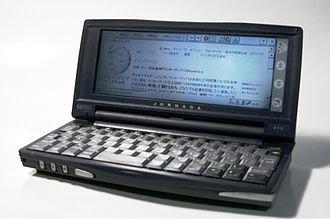
\includegraphics[width=0.8\textwidth]{330px-Jornada_690_HP_d.jpg} \\
  \caption[早期的智能手机]{HP Jornada 690開啟了手機和電腦結合的早期概念,成為智能手機早期概念典範。} 
  \label{fig:lengthscale}
\end{figure}

本章是第~\ref{cha:introduction}~章。下一节是~\ref{sec:challenge}。

\chapter{计划进度}
\begin{table}[h]
	\caption{计划进度}  
	\label{tab:schedule}
	\centering
	\scalebox{0.9}{
		\begin{tabular}{lll}
		  \toprule
		  \multicolumn{3}{c}{进度}\\
		  \midrule
		   2007.10~--~2008.05 & & 完成文献综述和开题报告\\
		  
		  2008.05~--~2008.07 & & 完成电渗流多尺度模拟的理论构建和初步模型验证,\\
		                   & & 同时开始写毕业论文\\
		  2008.07~--~2008.10 & & 完成模型验证,并进行多种条件下电渗流(泵)的仿真模拟,\\
		                    & & 实验数据处理,制表,论文书写\\
		  2008.10~--~2008.12 & & 完成所有仿真对象的模拟,并计划完成毕业论文的初稿\\
		  2008.12~--~2009.03 & & 完成论文修改\\
		  2009.03~--~2009.05  & & 准备答辩、答辩\\
		  \bottomrule
		\end{tabular}
	}
\end{table}

\begin{dotsequation}
    \begin{aligned}
		                     a&=b\\
		                     c&=d\\
		                  2x+y&=6\\
		                     x&=4y+\log (y)\\
		\sum_i^{10} i \times x&=y
    \end{aligned}
    \label{eq:log}
\end{dotsequation}

\section{研究现状及挑战}
\label{sec:challenge}
研究现状及挑战见~\autoref{eq:log},多个引用~\cite{Manz1990,Harrison1993,Erickson2003}。

\section{研究内容与论文结构}

研究内容\cite{erdHos1960evolution,konect:socialcomputing,konect}与论文结构\cite{Harrison1993,xiuwu2002,Erickson2003,Auroux2002}。

\chapter{算法}
尝试插入算法(见\autoref{alg:alg1})

\begin{algorithm}[h]
    \setstretch{1.3}
    \textbf{Input:} 两个数 $n$, $k$
    \begin{algorithmic}[1]
        \STATE 初始化 $s$ 为 $0$ \label{algline:init}
        \FOR{$i = 1,2,...,k$}    \COMMENT{\textbf{循环}}
        \label{algline:for} 
        \IF {$i\;\% \;5\neq 0$}
        \STATE $s=s+n+i$
        \ENDIF 
        \ENDFOR \label{algline:endfor}
        \STATE \textbf{return} $s$ \label{algline:return} 
    \end{algorithmic}
    \caption{sum($n$, $k$)}
    \label{alg:alg1}
\end{algorithm}

\chapter{代码}
尝试插入代码

\definecolor{commentColor}{rgb}{0.0, 0.5, 0.0}
\lstset{ %
    language=Python,                % the language of the code
    basicstyle=\scriptsize\ttfamily,           % the size of the fonts that are used for the code
    numbers=left,                   % where to put the line-numbers
    numberstyle=\tiny\color{gray},  % the style that is used for the line-numbers
    stepnumber=2,                   % the step between two line-numbers. If it's 1, each line 
    % will be numbered
    numbersep=5pt,                  % how far the line-numbers are from the code
    backgroundcolor=\color{white},      % choose the background color. You must add \usepackage{color}
    showspaces=false,               % show spaces adding particular underscores
    showstringspaces=false,         % underline spaces within strings
    showtabs=false,                 % show tabs within strings adding particular underscores
    rulecolor=\color{black},        % if not set, the frame-color may be changed on line-breaks within not-black text (e.g. commens (green here))
    tabsize=2,                      % sets default tabsize to 2 spaces
    captionpos=b,                   % sets the caption-position to bottom
    breaklines=true,                % sets automatic line breaking
    breakatwhitespace=false,        % sets if automatic breaks should only happen at whitespace
                 % show the filename of files included with \lstinputlisting;
    % also try caption instead of title
    keywordstyle=\color{blue},          % keyword style
    commentstyle=\color{commentColor},       % comment style
    stringstyle=\color{mauve},         % string literal style
    escapeinside={(*}{*)},            % if you want to add LaTeX within your code
    morekeywords={*,...}               % if you want to add more keywords to the set
}
\newcommand{\commentMath}[1]{$\color{commentColor}#1$}
\begin{lstlisting}
def func(n, k):
    """
    param n: 起始值 (*\commentMath{n}*)
    param k: 计数 (*\commentMath{k}*)
    """
    s=0
    for i in range(1,k):
        if i % 5 != 0:
            s = s+n+i
    return s
\end{lstlisting}




\jluReferenceFile{example}
\jluReferenceStyle{gbt7714-numerical} % gbt7714-author-year
\jluPrintReference



\begin{jluSelfIntroduction}
此处放置作者简介
\end{jluSelfIntroduction}



\begin{jluAcknowledgment}
三年时间看似漫长却又一晃而过,回首走过的岁月,我感慨良多。从最初的论文选题、思路梳理到研讨交流、反复修改直至最终完稿,都离不开老师、同学和亲人们的支持和无私帮助,在此我要向他们表达我最诚挚的谢意。

...

求学生涯暂告段落,但求知之路却永无止境。我将倍加珍惜大学生活给予我的珍贵财富,不忘初心,砥砺前行!
\end{jluAcknowledgment}

\appendix
\begin{appendices}
	\chapter{实验所用数据}
	......
	\chapter{其他}
	......
\end{appendices}

\end{document}
